\documentclass[a4paper]{article}
\usepackage[utf8]{inputenc}
\usepackage[spanish, es-tabla, es-noshorthands]{babel}
\usepackage[table,xcdraw]{xcolor}
\usepackage[a4paper, footnotesep = 1cm, width=22cm, top=2.5cm, height=25cm, textwidth=20cm, textheight=25cm]{geometry}
%\geometry{showframe}

\usepackage{tikz}
\usepackage{amsmath}
\usepackage{amsfonts}
\usepackage{amssymb}
\usepackage{float}
\usepackage{graphicx}
\usepackage{caption}
\usepackage{subcaption}
\usepackage{multicol}
\usepackage{multirow}
\usepackage{wrapfig}
\setlength{\doublerulesep}{\arrayrulewidth}
\usepackage{booktabs}

\usepackage{hyperref}
\hypersetup{
    colorlinks=true,
    linkcolor=blue,
    filecolor=magenta,      
    urlcolor=blue,
    citecolor=blue,    
}

\newcommand{\note}[1]{
	\begin{center}
		\huge{ \textcolor{red}{#1} }
	\end{center}
}

\setcounter{topnumber}{2}
\setcounter{bottomnumber}{2}
\setcounter{totalnumber}{4}
\renewcommand{\topfraction}{0.85}
\renewcommand{\bottomfraction}{0.85}
\renewcommand{\textfraction}{0.15}
\renewcommand{\floatpagefraction}{0.8}
\renewcommand{\textfraction}{0.1}
\setlength{\floatsep}{5pt plus 2pt minus 2pt}
\setlength{\textfloatsep}{5pt plus 2pt minus 2pt}
\setlength{\intextsep}{5pt plus 2pt minus 2pt}

\newcommand{\quotes}[1]{``#1''}
\usepackage{array}
\newcolumntype{C}[1]{>{\centering\let\newline\\\arraybackslash\hspace{0pt}}m{#1}}
\usepackage[american]{circuitikz}
\usetikzlibrary{calc}
\usepackage{fancyhdr}
\usepackage{units} 

\graphicspath{{../Ejercicio-1/}{../Ejercicio-2/}{../Ejercicio-3/}{../Ejercicio-4/}{../ParteI/}{../ParteII/}{../ParteIII/}{../ParteIV/}}

\pagestyle{fancy}
\fancyhf{}
\lhead{22.14 - Electrónica IV}
\rhead{Mechoulam, Lambertucci, Londero}
\rfoot{Página \thepage}


\begin{document}

%%%%%%%%%%%%%%%%%%%%%%%%%
%		Caratula		%
%%%%%%%%%%%%%%%%%%%%%%%%%


%%%%%%%%%%%%%%%%%%%%%
%		Indice		%
%%%%%%%%%%%%%%%%%%%%%


%%%%%%%%%%%%%%%%%%%%%
%		Informe		%
%%%%%%%%%%%%%%%%%%%%%


\section{Mediciones del circuito físico}
Se armó una fuente boost en protoboard con las siguientes especificaciones para su modo continuo:
\begin{itemize}
\item L=40 $\mu$Hy
\item $R_g$=100 $\Omega$
\item $R_L$=147 $\Omega$
\item $C$ = 47 $\mu$F
\item $M_1$ = IRF540
\item $D$ = MUR160
\item $R_{shunt}$=5 $\Omega$
\item Transistores BJT: BC-337 y BC-327
\item $V_d$ = 12 V
\item D=0.23 (Waveform)
\item $f_{switching}$ = 170 KHz
\end{itemize}
Se utilizó una resistencia de shunt para medir la corriente por la bobina.
Con los valores provistos arriba se obtuvo una tensión de salida $V_o \approx 20 \ V$ y se midieron las siguientes señales:



\begin{figure}[H]
	\centering
	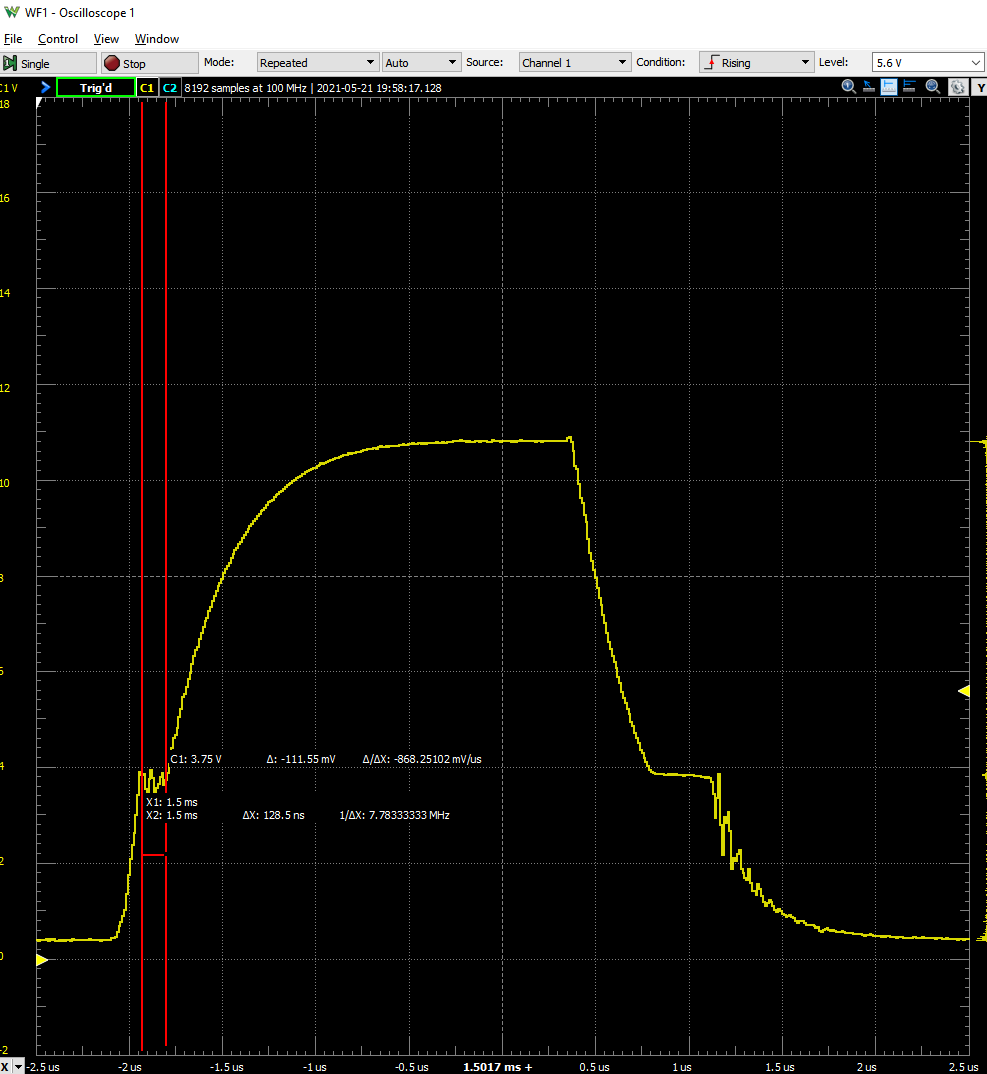
\includegraphics[width=\linewidth]{Imagenes/Continuo_VGS}
	\caption{Modo continuo: Tensión $V_{GS}$.}
	\label{fig:Cont_VGS}
\end{figure}


\begin{figure}[H]
	\centering
	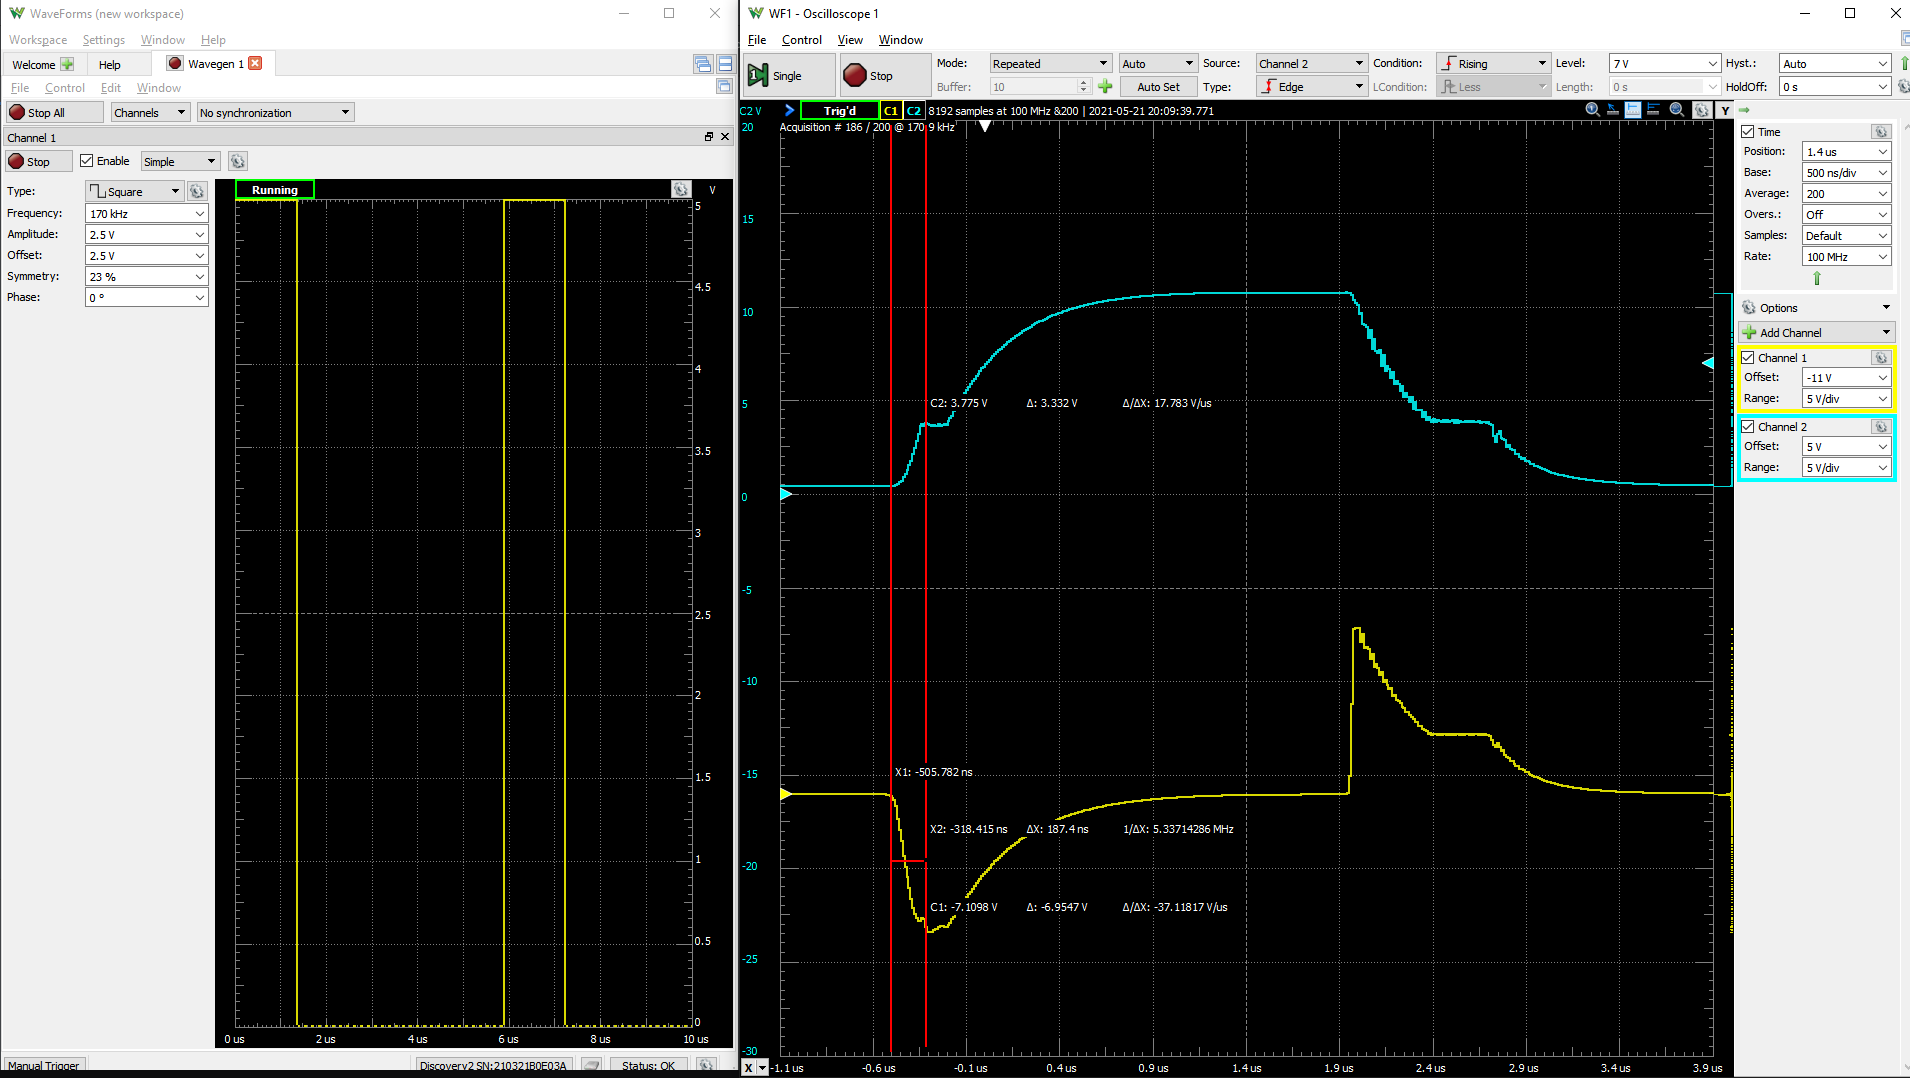
\includegraphics[width=\linewidth]{Imagenes/Continuo_VGS_IG}
	\caption{Modo continuo: Tensión $V_{GS}$ e $I_{GS}$.}
	\label{fig:CONT_VGS_IGS}
\end{figure}

\begin{figure}[H]
	\centering
	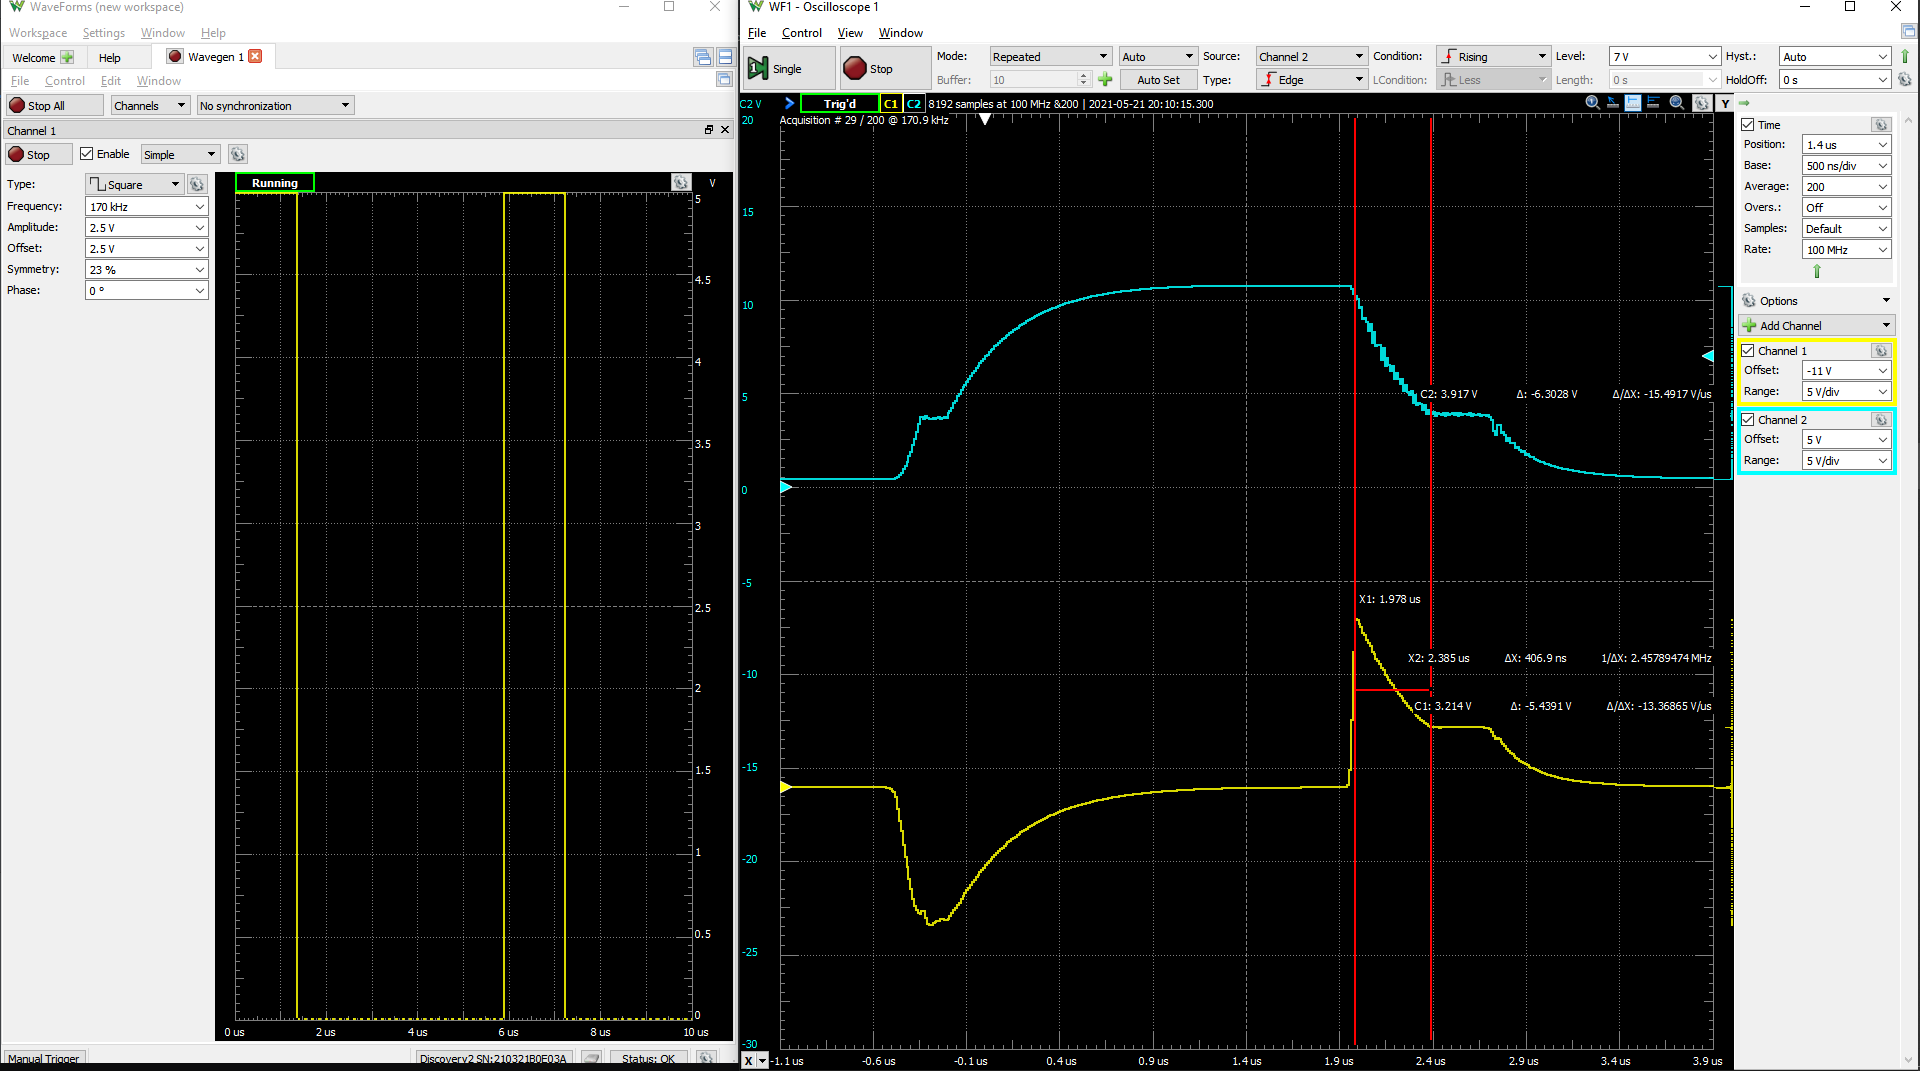
\includegraphics[width=\linewidth]{Imagenes/Continuo_VGS_IG_2}
	\caption{Modo continuo: $V_{GS}$ e $I_{GS}$ detalle.}
	\label{fig:CONT_VGS_IGS_2}
\end{figure}

\begin{figure}[H]
	\centering
	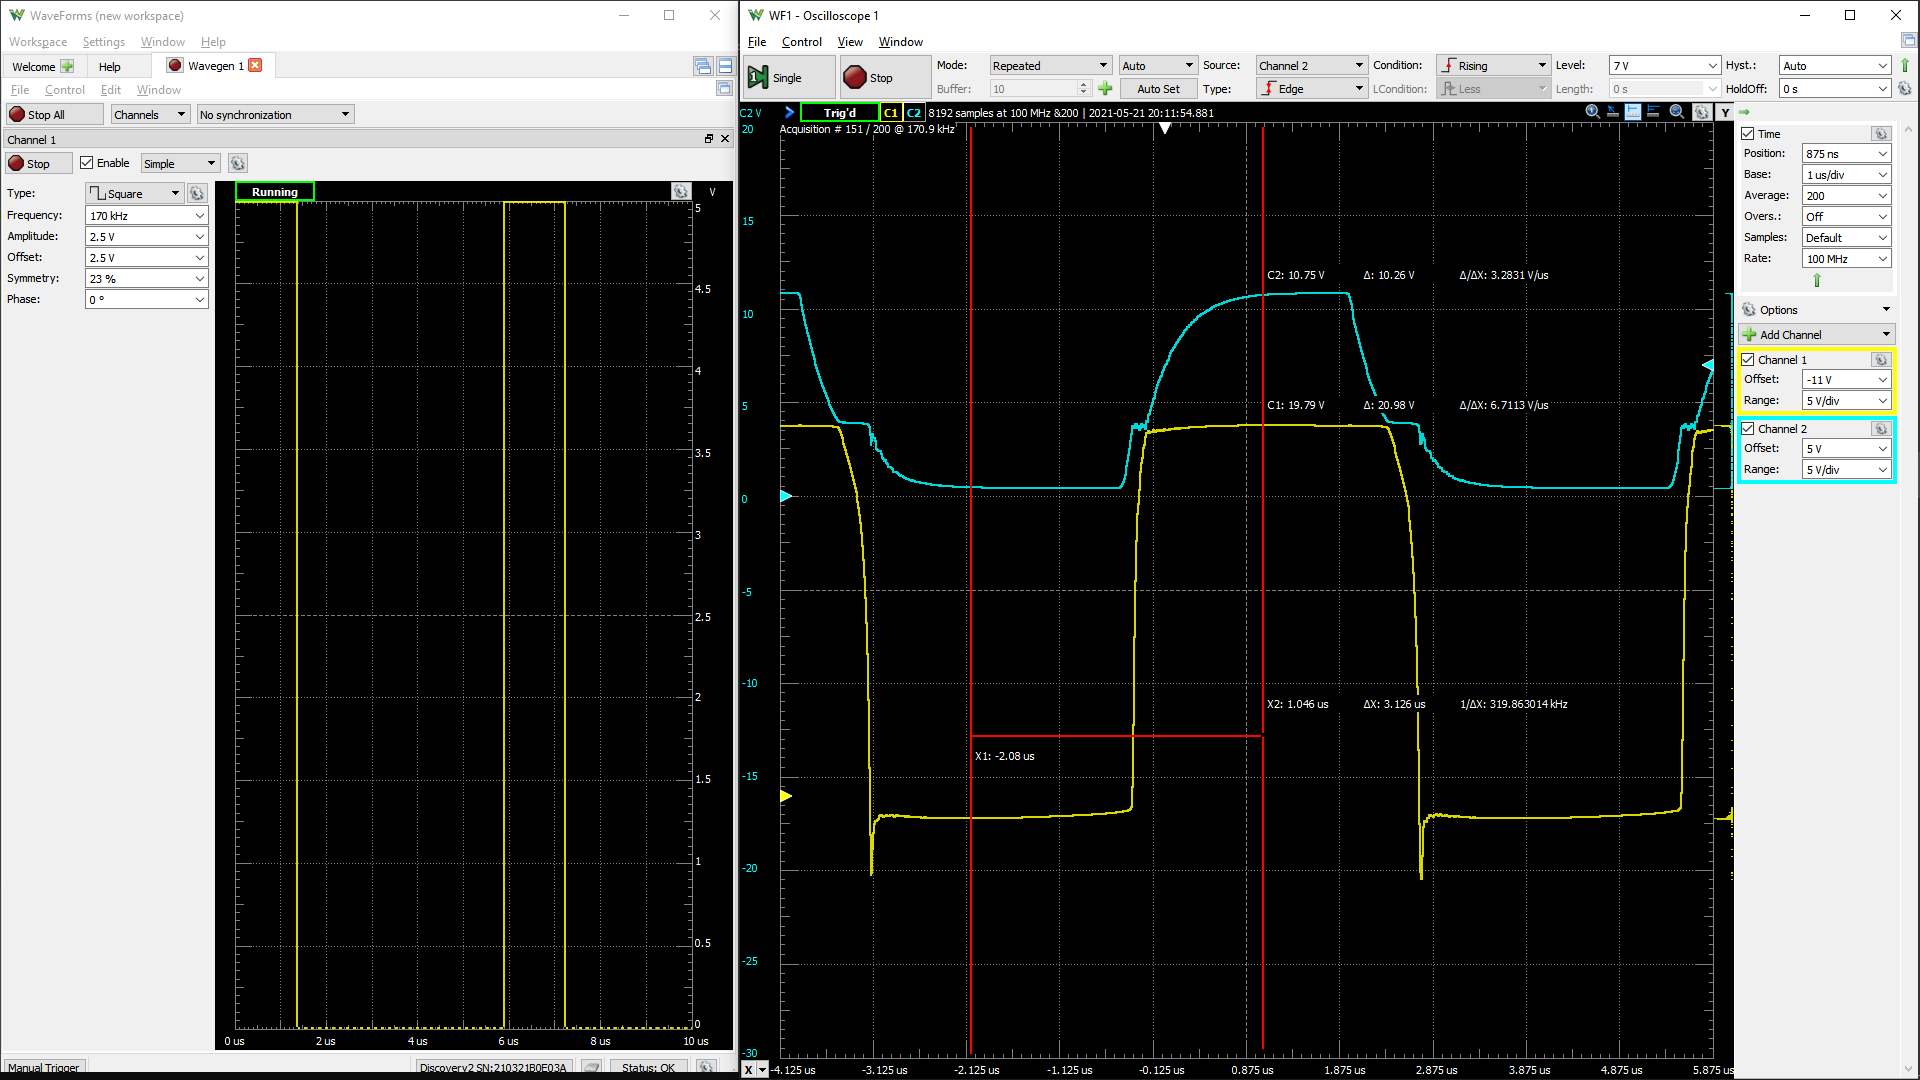
\includegraphics[width=\linewidth]{Imagenes/Continuo_VGS_VDiodo}
	\caption{Modo continuo: $V_{GS}$ y $V_D$.}
	\label{fig:CONT_VGS_VD}
\end{figure}

\begin{figure}[H]
	\centering
	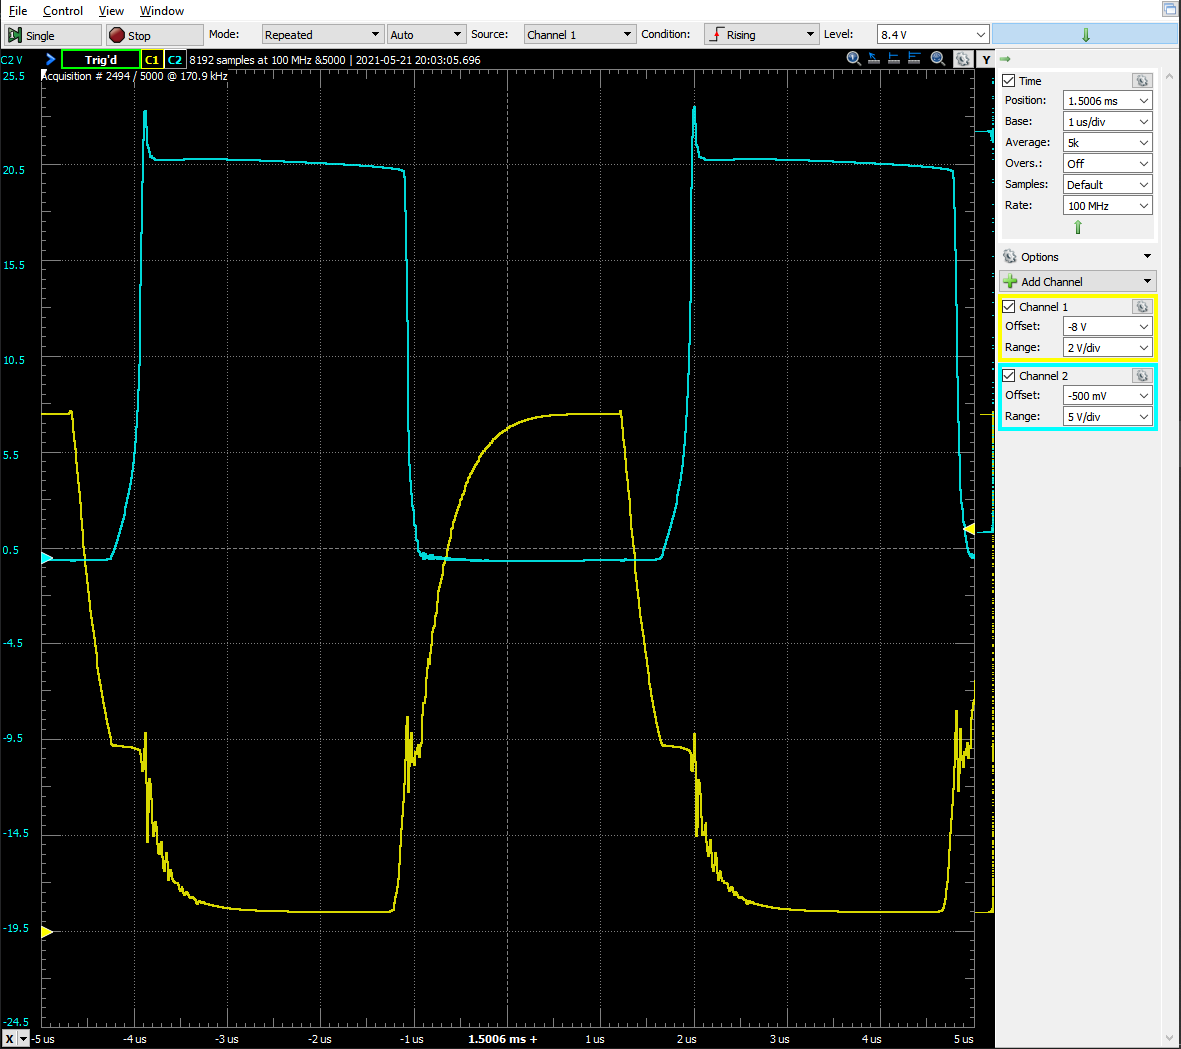
\includegraphics[width=\linewidth]{Imagenes/Continuo_VGS_VDS}
	\caption{Modo continuo: $V_{GS}$ y $V_{DS}$.}
	\label{fig:CONT_VGS_VDS}
\end{figure}

\begin{figure}[H]
	\centering
	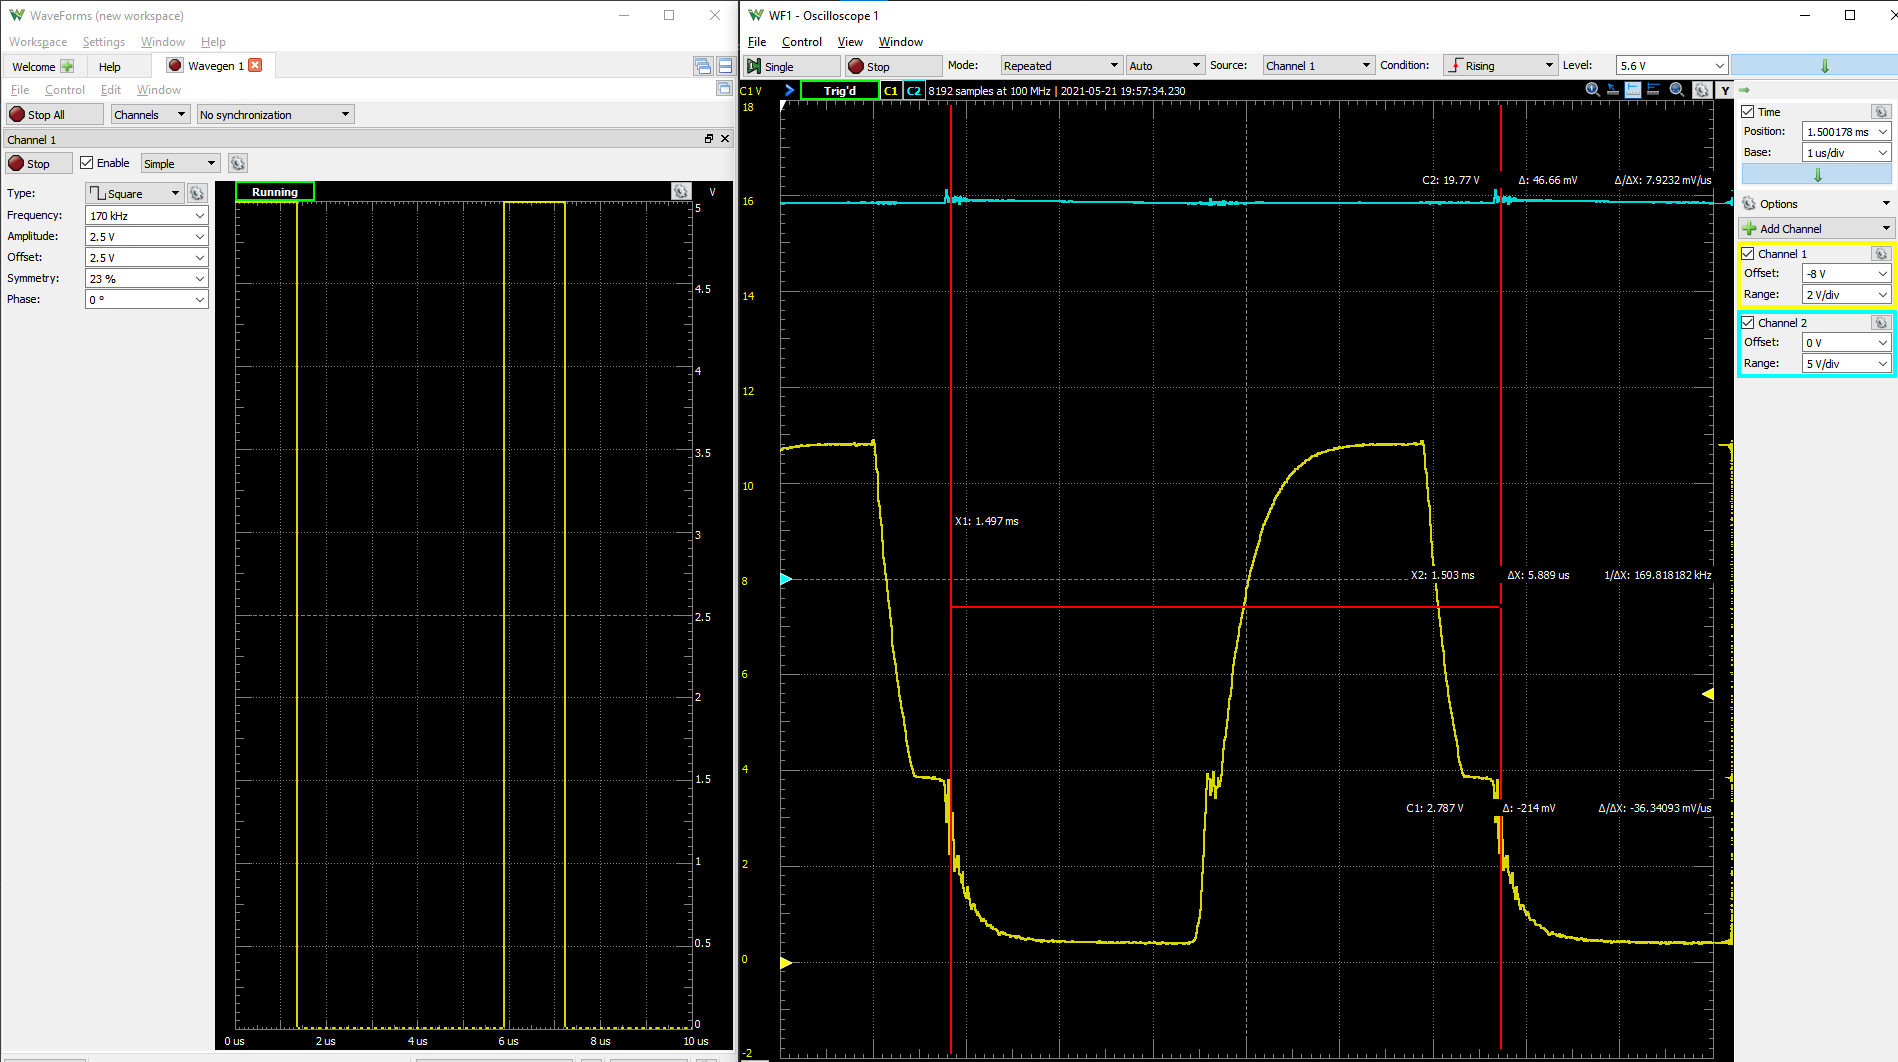
\includegraphics[width=\linewidth]{Imagenes/Continuo_VGS_VO}
	\caption{Modo continuo: $V_{GS}$ y $V_o$.}
	\label{fig:CONT_VGS_VO}
\end{figure}
\begin{figure}[H]
	\centering
	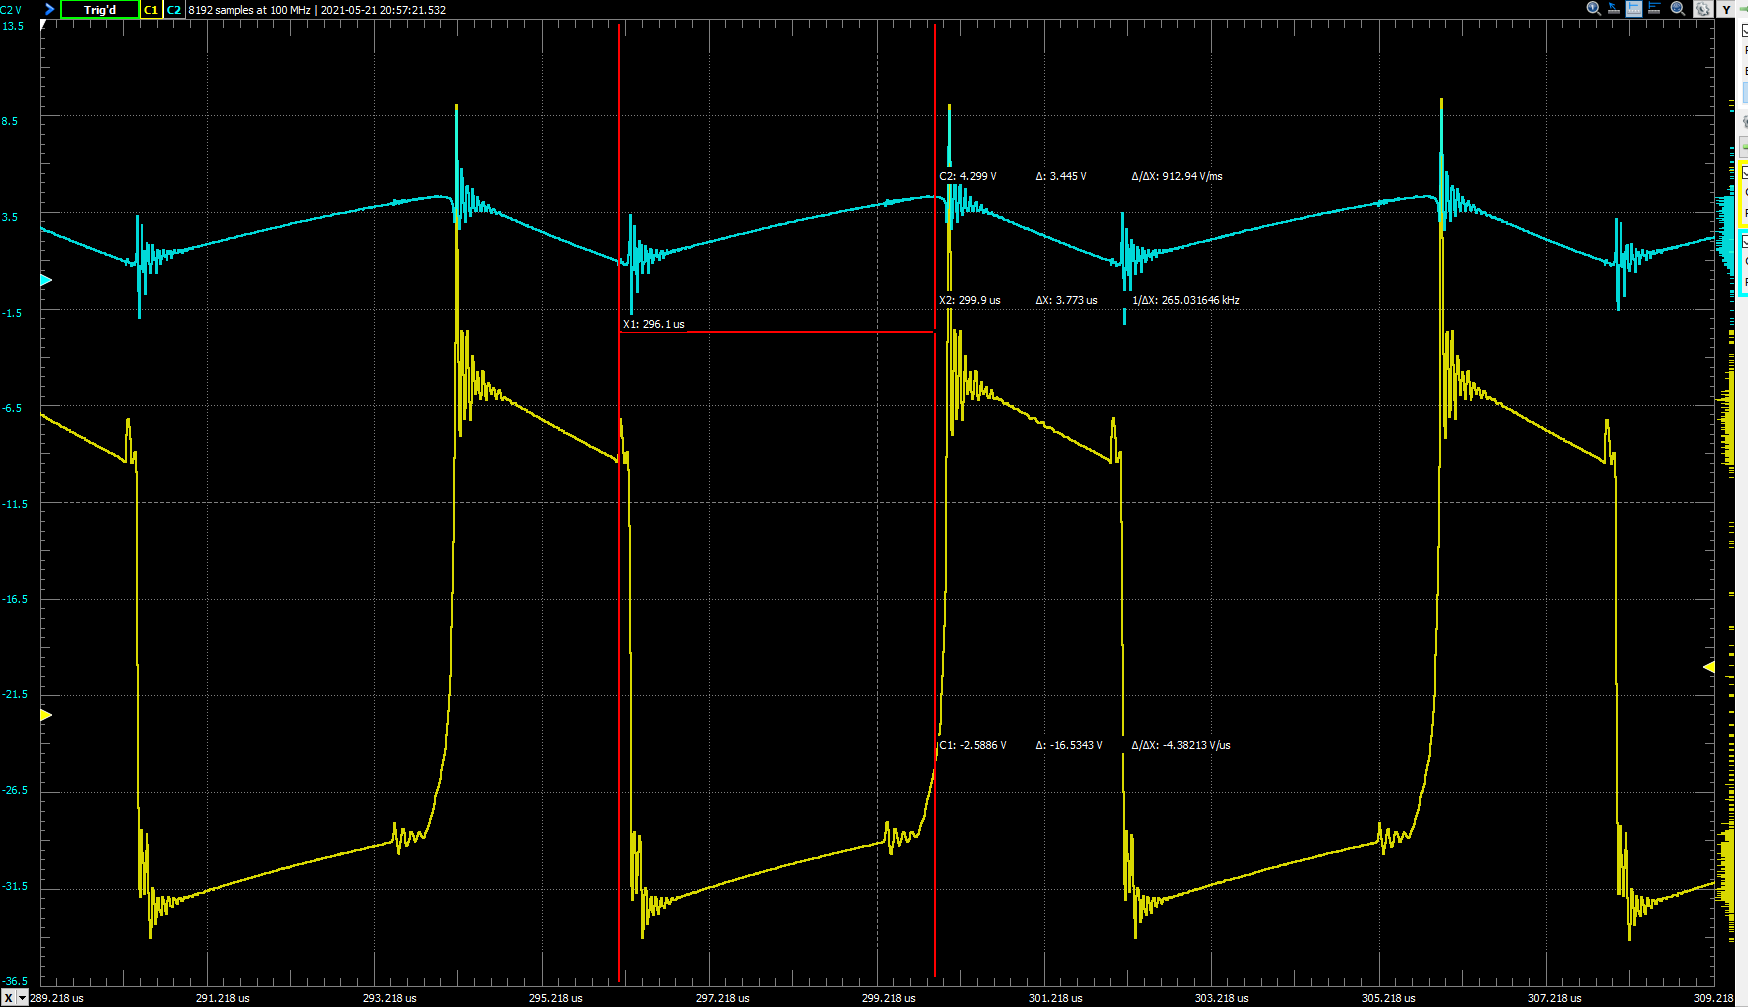
\includegraphics[width=\linewidth]{Imagenes/Continuo_VL_IL}
	\caption{Modo continuo: $V_L$ y $I_L$.}
	\label{fig:CONT_VL_IL}
\end{figure}




Luego para el modo discontinuo lo que se hizo fue aumentar la carga  hasta los $R_L=220 \ \Omega$ y cambiar el dutycycle hasta $D=40\%$(Analog)
obteniendo los siguientes gráficos

\begin{figure}[H]
	\centering
	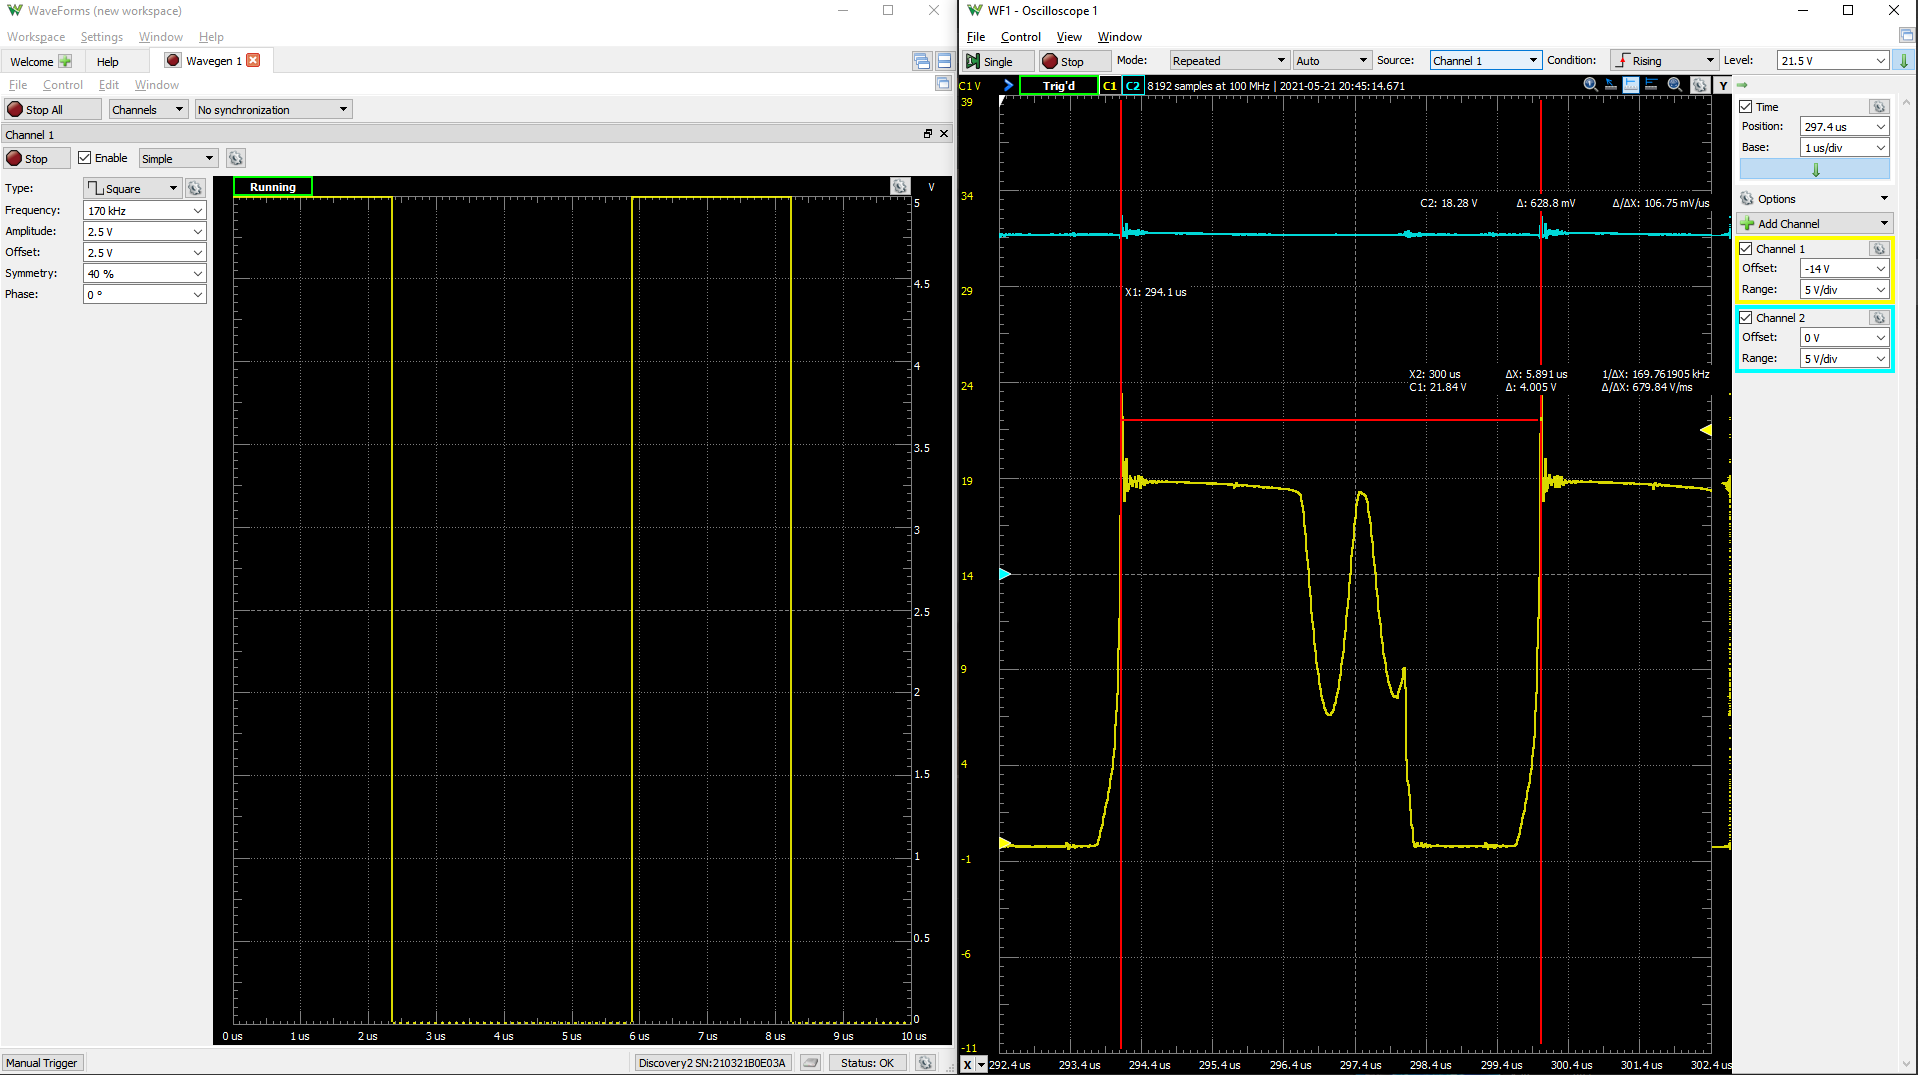
\includegraphics[width=\linewidth]{Imagenes/Discontinuo_VDS_VO}
	\caption{Modo discontinuo: $V_{DS}$ y $V_o$.}
	\label{fig:DISCONT_VDS_VO}
\end{figure}
\begin{figure}[H]
	\centering
	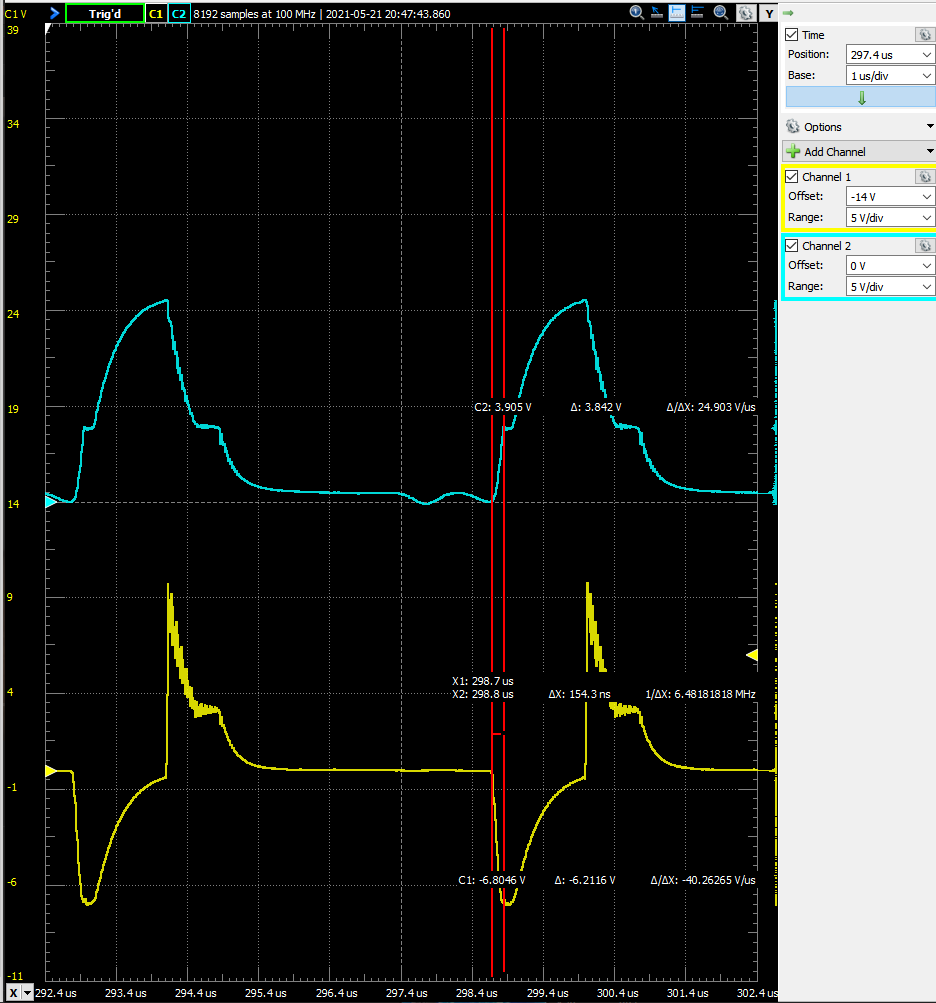
\includegraphics[width=\linewidth]{Imagenes/Discontinuo_VGS_IG}
	\caption{Modo discontinuo: $V_{GS} e I_G $.}
	\label{fig:DISC_VGS_IG}
\end{figure}
\begin{figure}[H]
	\centering
	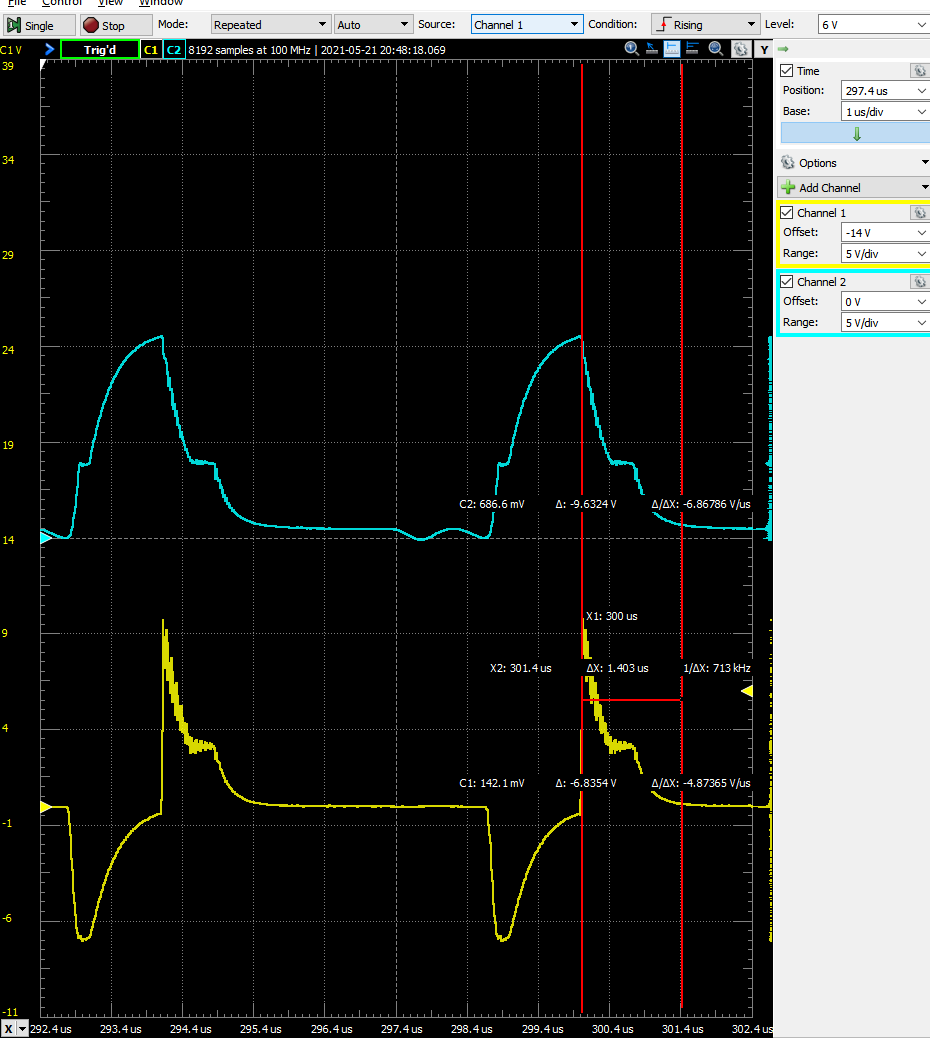
\includegraphics[width=\linewidth]{Imagenes/Discontinuo_VGS_IG_2}
	\caption{Modo discontinuo: $V_{GS} e I_G $ detalle.}
	\label{fig:DISC_VGS_IG_2}
\end{figure}
\begin{figure}[H]
	\centering
	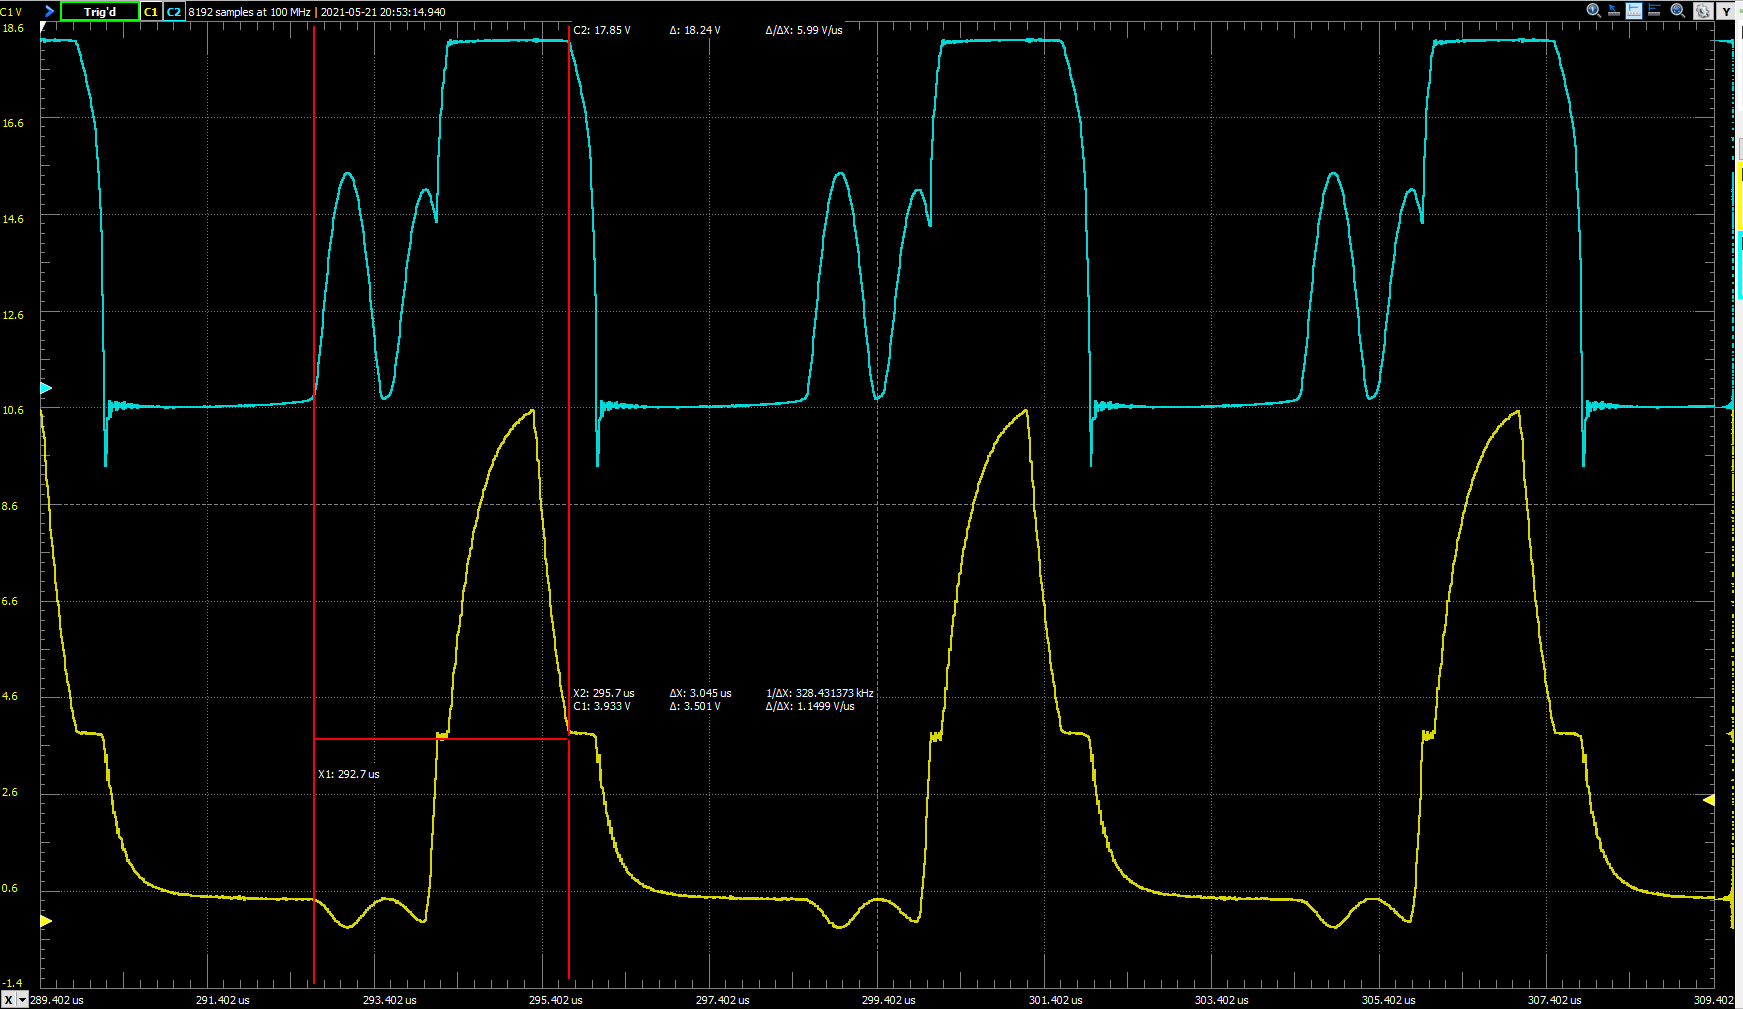
\includegraphics[width=\linewidth]{Imagenes/Discontinuo_VGS_VDiodo}
	\caption{Modo discontinuo: $V_{GS}$ y $V_D$.}
	\label{fig:DISC_VGS_VD}
\end{figure}
\begin{figure}[H]
	\centering
	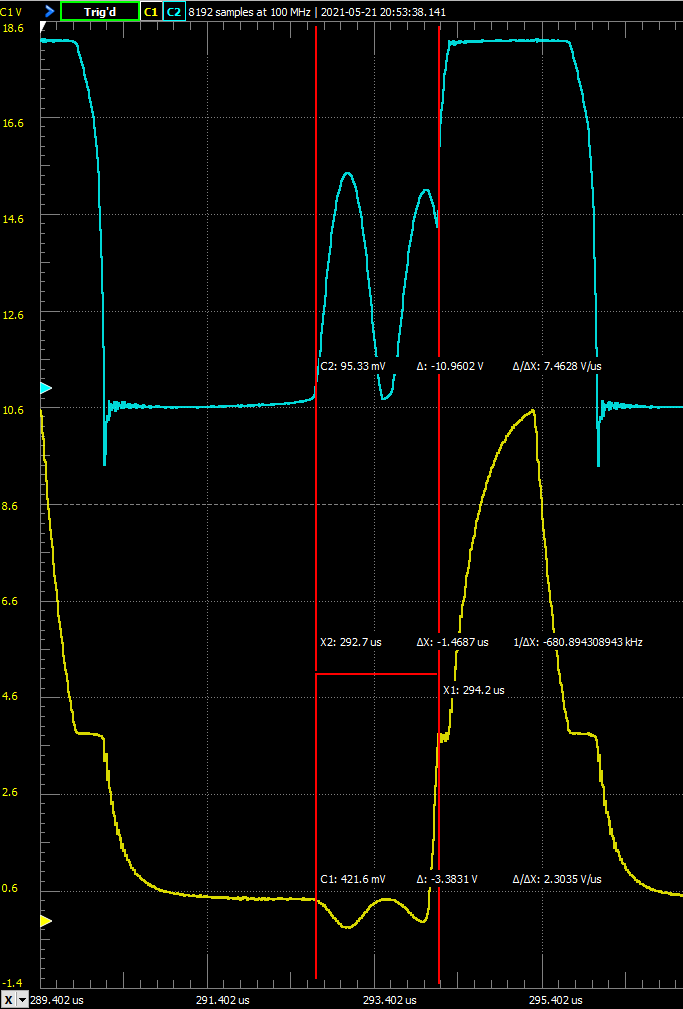
\includegraphics[width=\linewidth]{Imagenes/Discontinuo_VGS_VDiodo_2}
	\caption{Modo discontinuo: $V_{GS}$ y $V_D$ detalle.}
	\label{fig:DISC_VGS_VD_2}
\end{figure}
\begin{figure}[H]
	\centering
	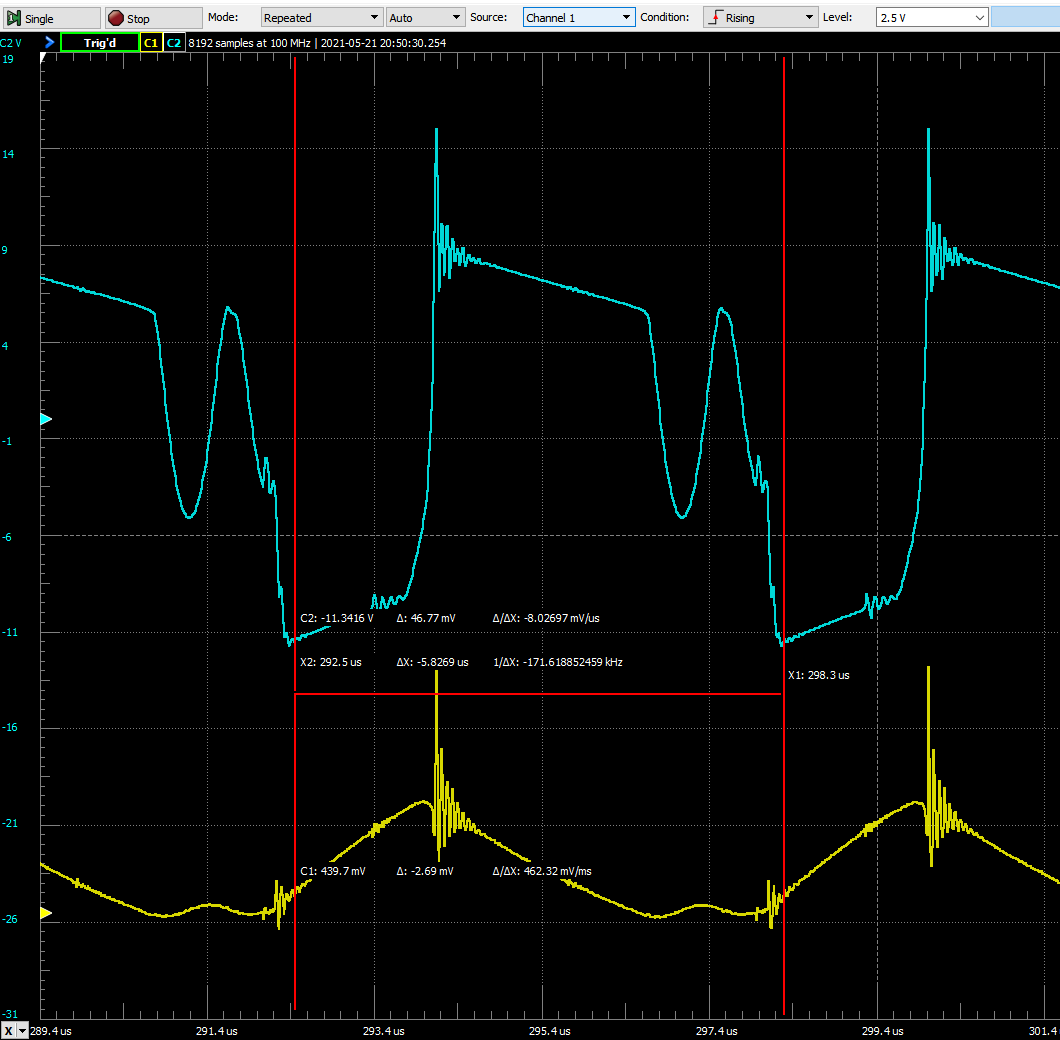
\includegraphics[width=\linewidth]{Imagenes/Discontinuo_VL_IL_1}
	\caption{Modo discontinuo: $V_L$ e $I_L$.}
	\label{fig:DISC_VL_IL}
\end{figure}


\begin{figure}[H]
	\centering
	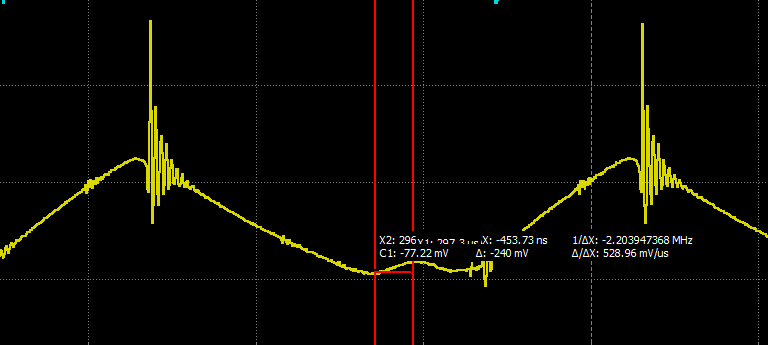
\includegraphics[width=\linewidth]{Imagenes/Discontinuo_VL_IL_2}
	\caption{Modo discontinuo: $V_L$ e $I_L$ detalle 1.}
	\label{fig:DISC_VL_IL_2}
\end{figure}
\begin{figure}[H]
	\centering
	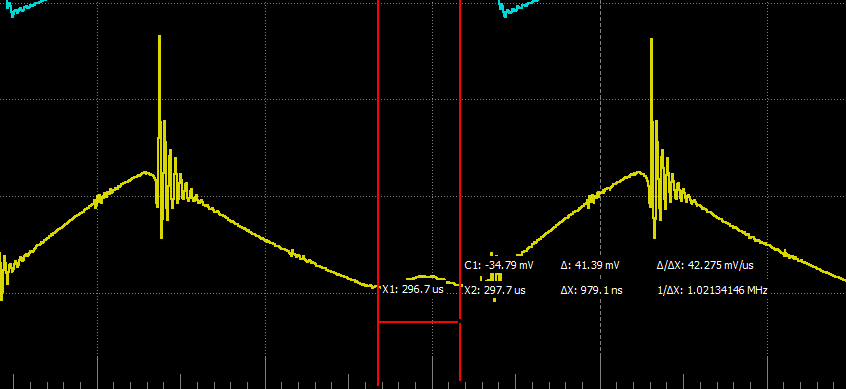
\includegraphics[width=\linewidth]{Imagenes/Discontinuo_VL_IL_3}
	\caption{Modo discontinuo: $V_L$ e $I_L$ detalle 2.}
	\label{fig:DISC_VL_IL_3}
\end{figure}

Tambien se notaron algunas particularidades en la propagación de las señales por el driver para el MOS, como que el duty del analog no resulta ser el complemento del que se encuentra en la salida del totempole debido a que 
\begin{figure}[H]
	\centering
	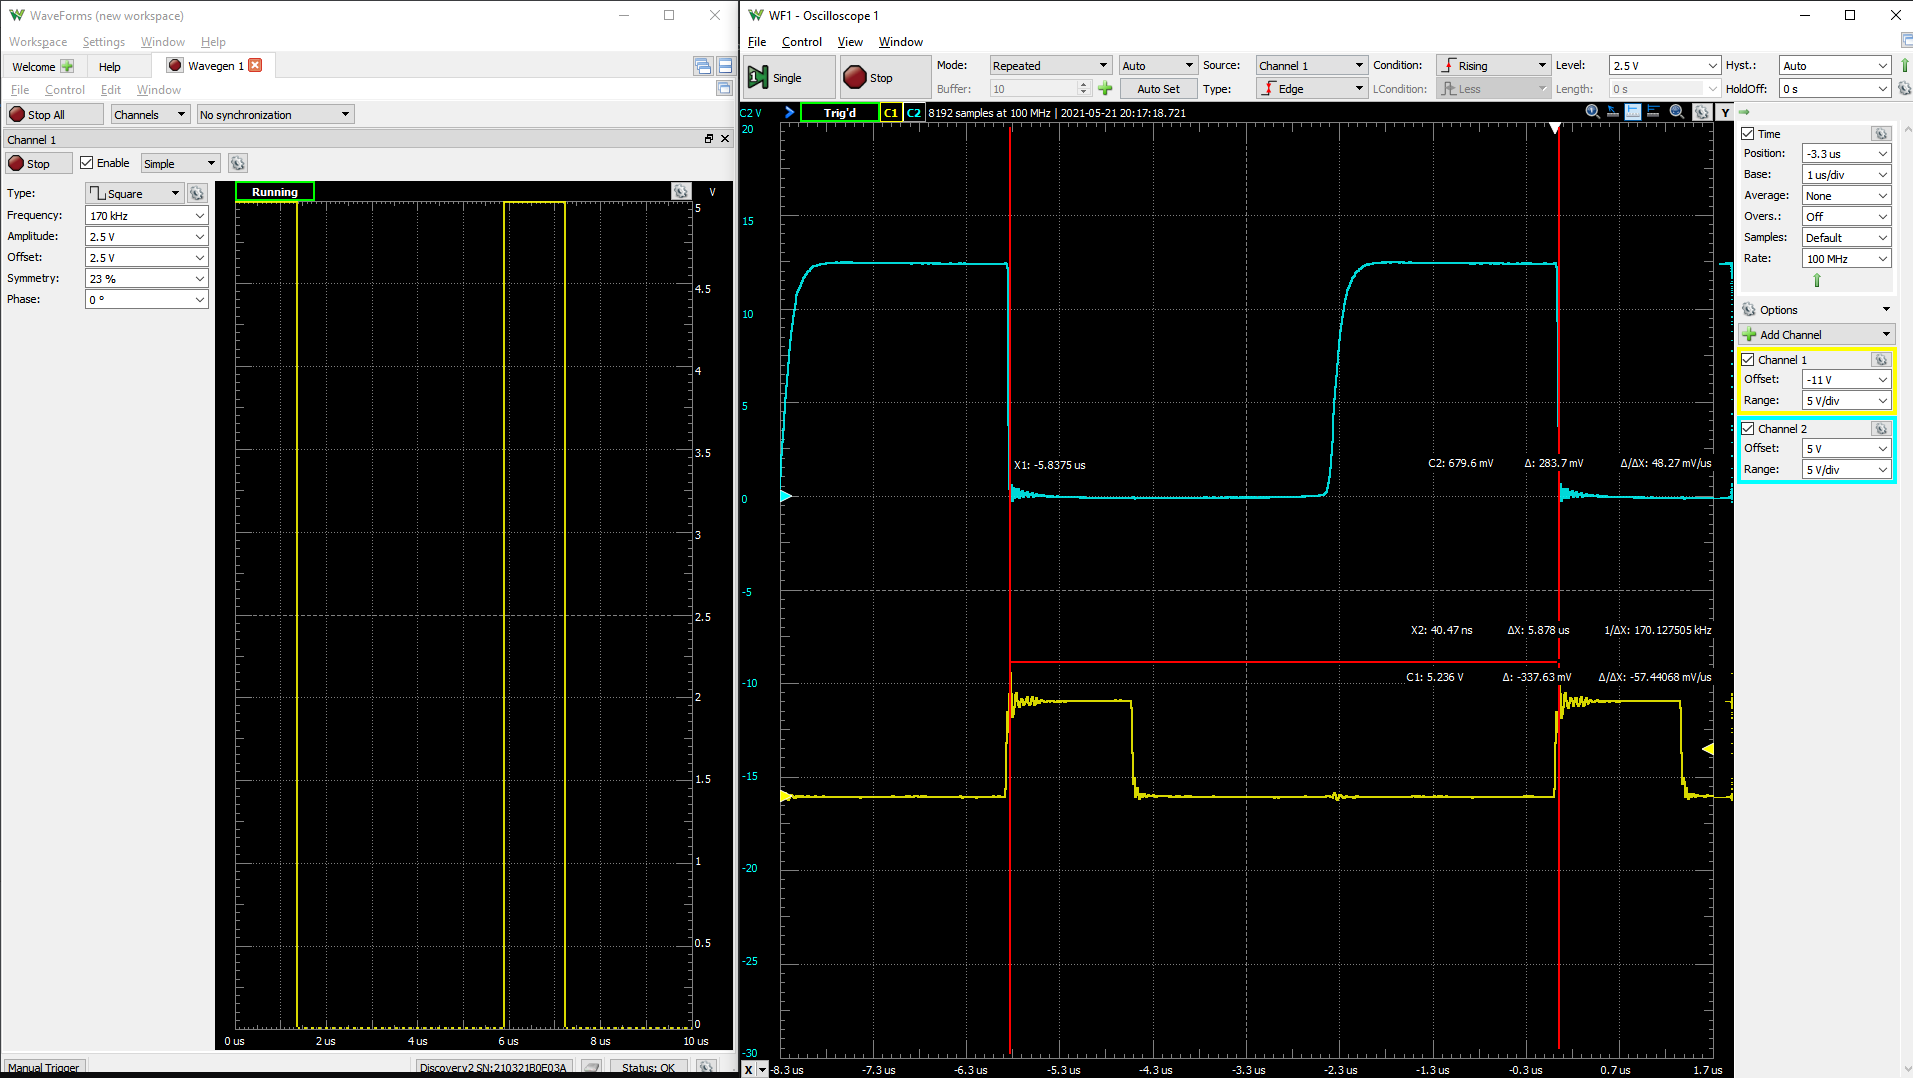
\includegraphics[width=\linewidth]{Imagenes/V_A_V_emisor_comun}
	\caption{Propagación señal de disparo 1.}
	\label{fig:VAVE1}
\end{figure}

\begin{figure}[H]
	\centering
	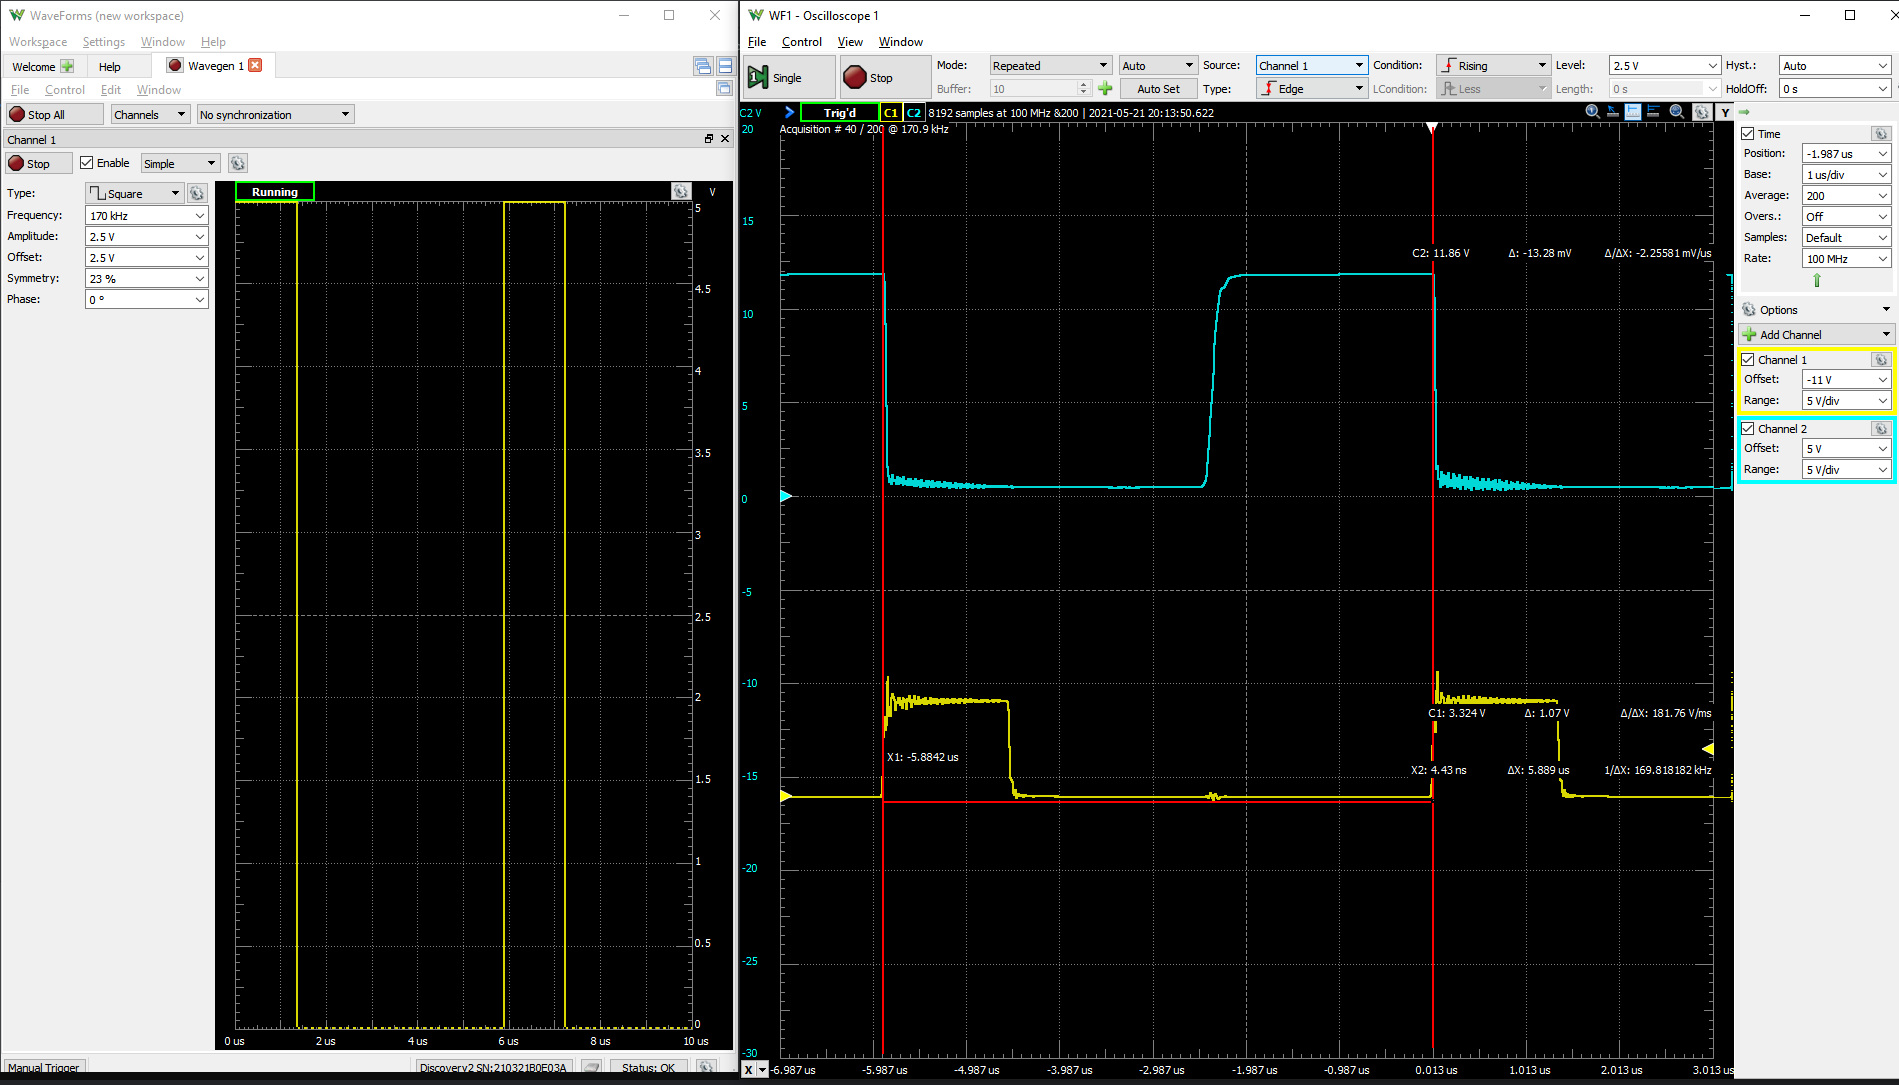
\includegraphics[width=\linewidth]{Imagenes/V_A_V_TTpole}
	\caption{Propagacion señal totempole.}
	\label{fig:VAVTTP}
\end{figure}
\begin{figure}[H]
	\centering
	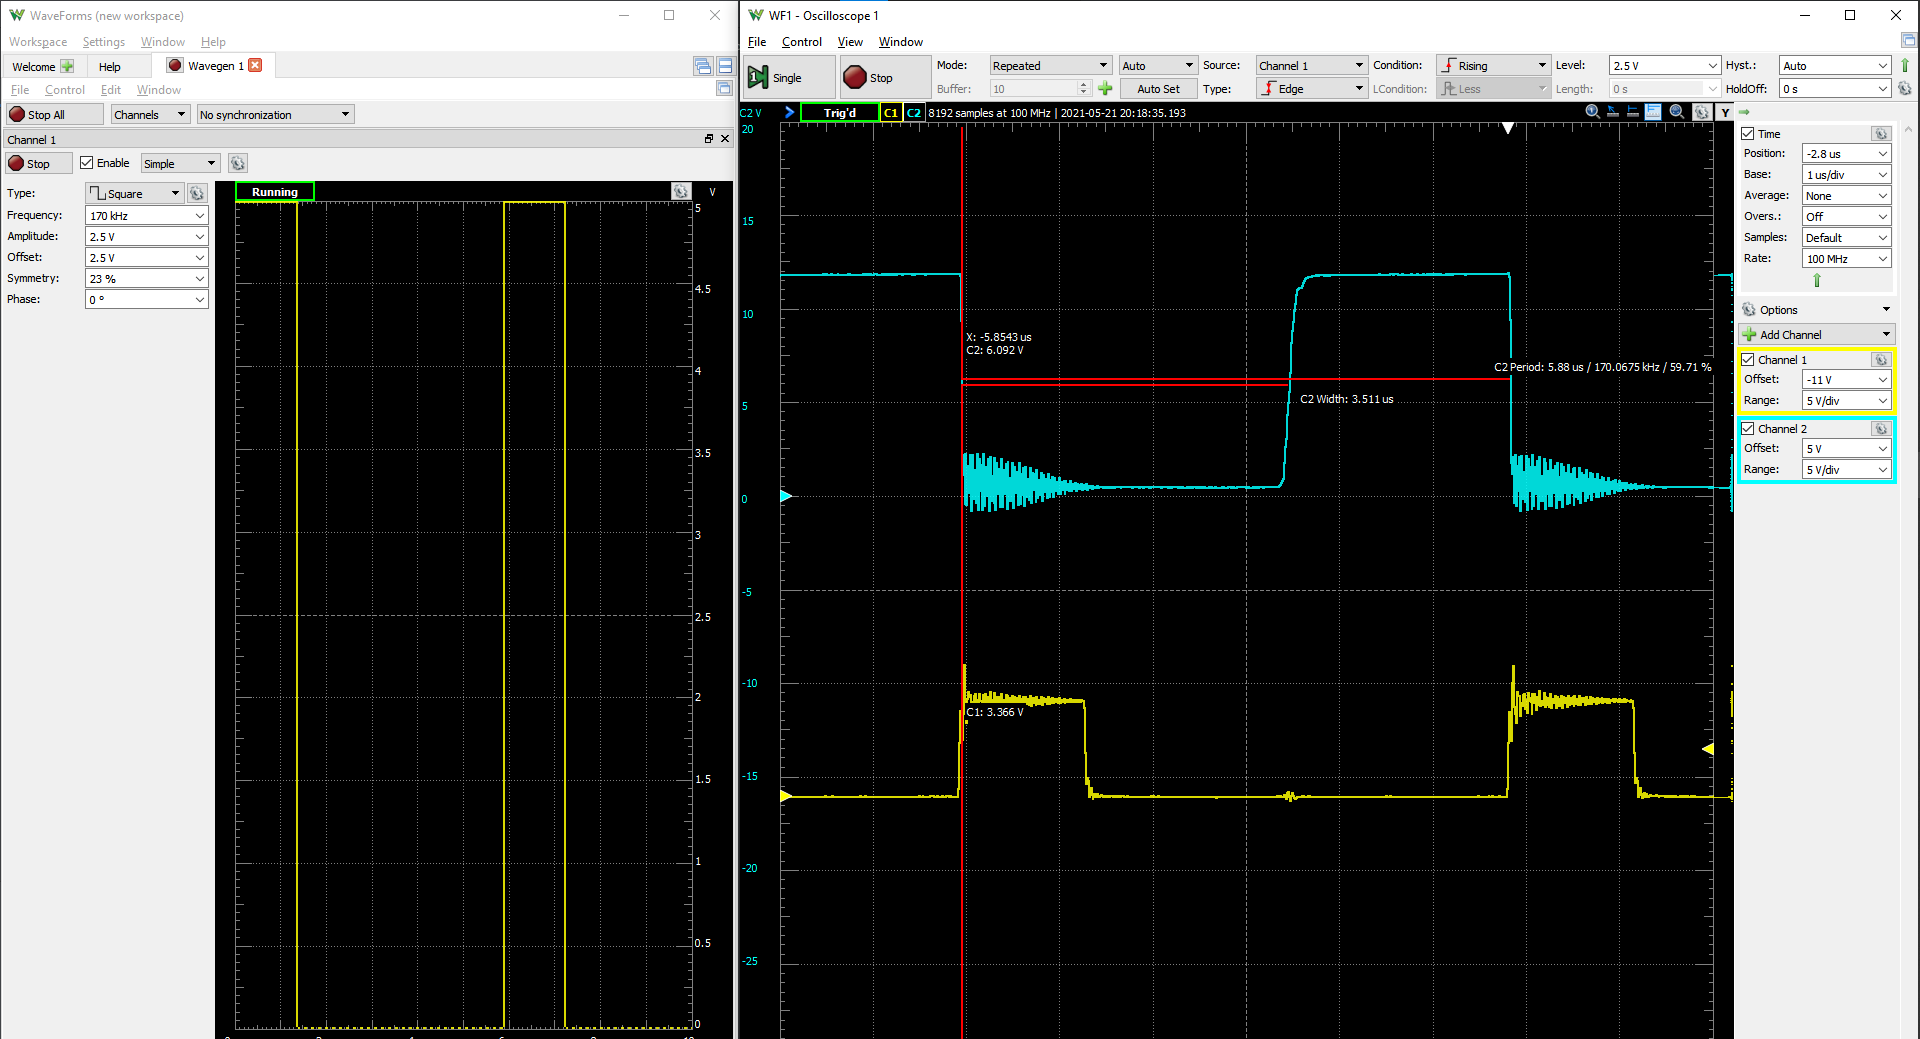
\includegraphics[width=\linewidth]{Imagenes/V_A_V_TTpole_detalle_1}
	\caption{Medición  dutycycle Totempole.}
	\label{fig:MED_TTP}
\end{figure}
\begin{figure}[H]
	\centering
	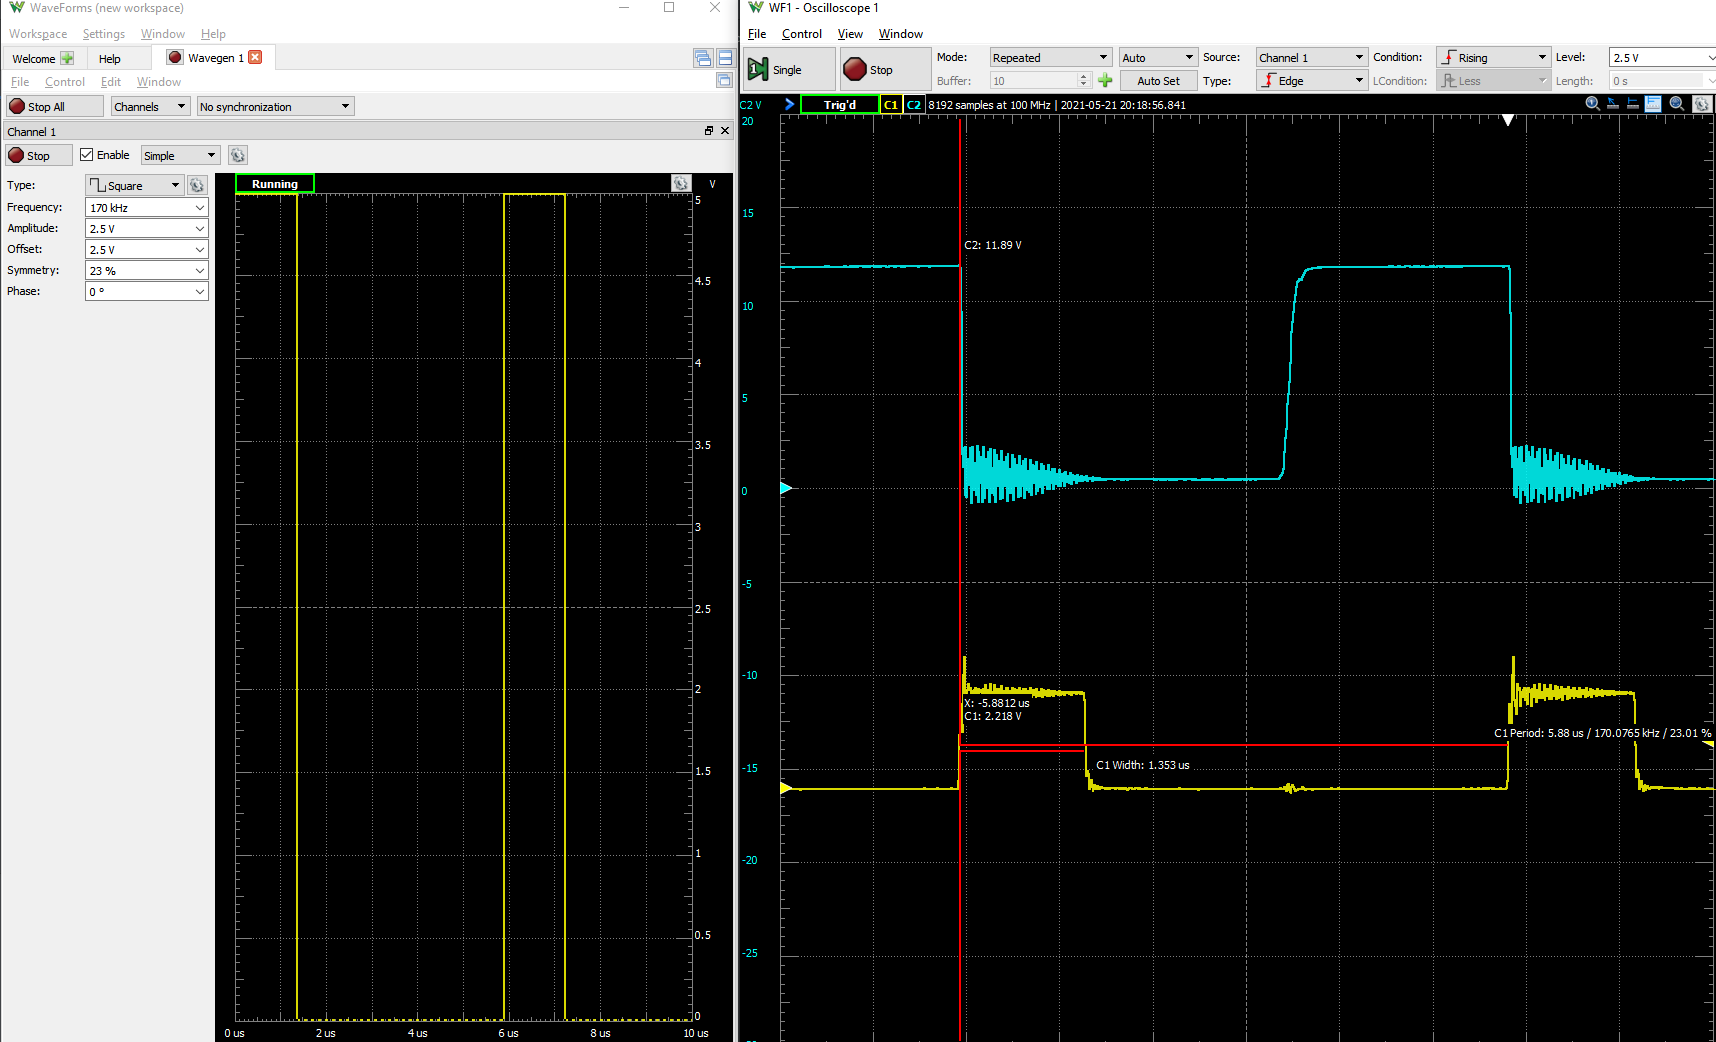
\includegraphics[width=\linewidth]{Imagenes/V_A_V_TTpole_detalle_2}
	\caption{Medición  dutycycle analog.}
	\label{fig:MED_ANAL}
\end{figure}

\end{document}
